\chapter{Обзор существующих решений рассматриваемой задачи или её модификаций}
\label{cha:ch_2}
В первую очередь рассмотрим уже упомянутую работу о детекции эффекта 
Сюняева-Зельдовича \cite{Bonjean}. Её автор использует для сегментации данных архитектуру U-net 
(эта архитектура будет использоваться и в этой работе). \\

Основной целью описываемой работы являлось создание алгоритма для детекции источников через эффект 
Сюняева-Зельдовича по данным телескопа <<Планк>>. Соответственно, кроме самих обзоров неба, полученных 
<<Планком>>, использовались еще три каталога скоплений для создания целевых данных:

\begin{enumerate}
	\item PSZ2. Этот каталог был получен по данным <<Планка>>  при помощи алгоритмов 
	согласованного мультифильтра и PowellSnakes.
	\item MCXC (Meta-Catalogue of X-ray detected Clusters). Это объединенный каталог из всех 
	других каталогов скоплений, полученных из данных телескопа ROSAT.
	\item RedMaPPer (Red-sequence Matched-filter Probabilistic Percolation). Каталог скоплений, 
	полученный с помощью одноимённого алгоритма из данных оптического диапазона.
\end{enumerate}

В описываемой работе для создания тренировочных выборок использовалось разбиение неба проекцией 
HEALPix (Hierarchical Equal Area isoLatitude Pixelisation). \\
\begin{figure}[h]
	\center{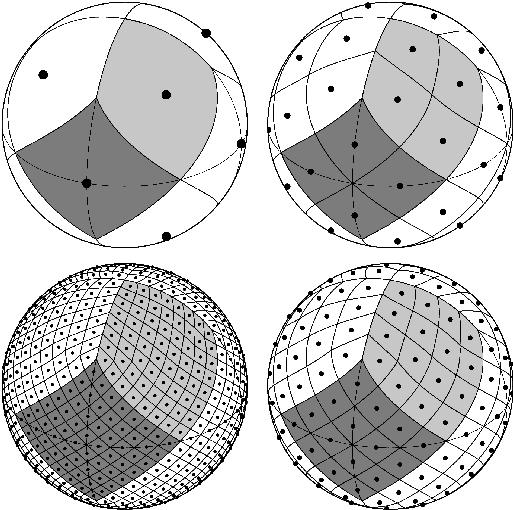
\includegraphics[width=5cm]{healpix0}}
	\caption{Примеры разбиения сферы HEALPix \cite{Healpix}}
\end{figure}

Разбиение с параметром $n_{side}=2$ позволяет получить 48 больших областей неба. Некоторые из них 
были использованы для тестирования полученной модели и для валидации, все остальные были 
использованы для обучения модели.\\ 

Случайным образом в соответствуюхих областях разбиения HEALPix выбирались центры патчей и их 
ориентации для создания тренировочных, валидационных и тестовых выборок. Каждый патч представлял 
из себя изображение размера 64 x 64 с шестью каналами различных данных. Размер каждого пикселя 
на таких патчах составлял 1.7 arcmin. \\

После этого 100000 патчей были использованы для обучения нейросети. Обучение длилось более 30 эпох. \\ 
\begin{figure}[h!]
	\center{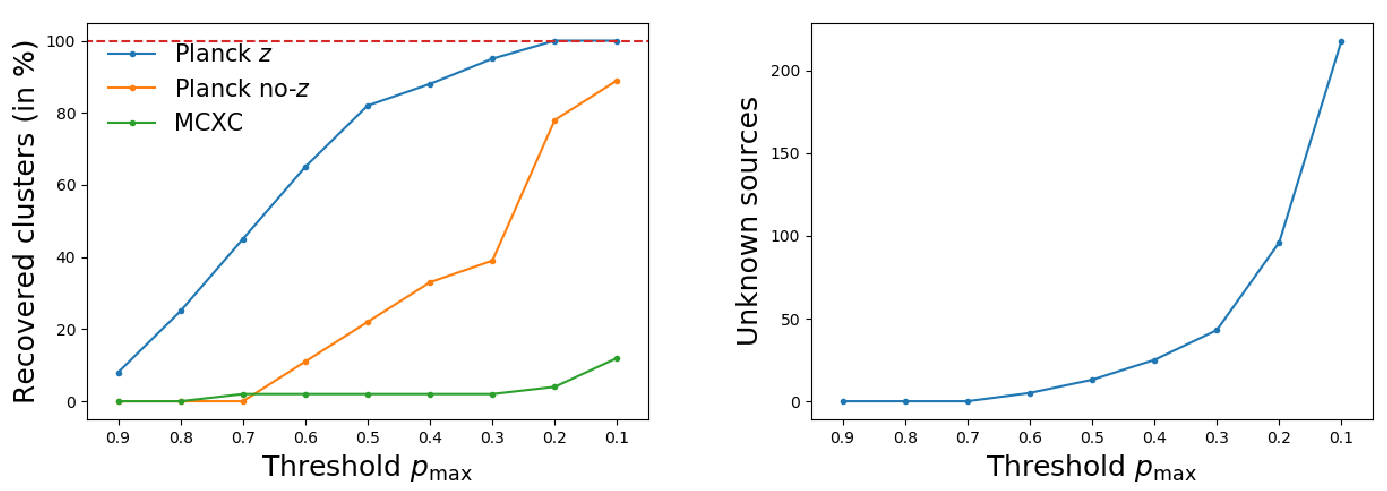
\includegraphics[width=15cm]{sz0}}
	\caption{Результаты исследования работы \cite{Bonjean}}
\end{figure}

Для детекции скоплений на полученных из нейросети данный, зонами скоплений обозначались зоны, 
занимающие пиксели со значением больше $p_{max}$, а затем на них находились барицентры, которые 
впоследствии считались предсказанными центрами скоплений. Таким образом большая часть скоплений из 
каталога PS2 была успешно распознана нейросетью. \\
